%% Report on mu -> e gamma in the S3-3HDM: exact and soft-broken vacua.
%% Companion: derivations_07.tex (the derivation ledger, auto-generated by the notebook).
%% Source: research/thdm_s3/07_mu_to_e_gamma.ipynb
\documentclass[11pt,a4paper]{article}
\usepackage[T1]{fontenc}
\usepackage[utf8]{inputenc}
\usepackage{amsmath,amssymb}
\usepackage{graphicx}
\usepackage{booktabs}
\usepackage[margin=2.4cm]{geometry}
\usepackage[colorlinks=true,linkcolor=blue,citecolor=blue,urlcolor=blue]{hyperref}
% Generated by report_numbers.py from results/*.json -- do not edit by hand.
% Use as \macro{} in text; the sample sizes belong in maths mode.
\newcommand{\nExactPoints}{1973}  % points surviving the exact-S3 scan (viable_points.json: n_points)
\newcommand{\nExactSample}{6\times10^{7}}  % points sampled in the exact-S3 scan (use in maths mode) (viable_points.json: sample_size)
\newcommand{\nSoftPoints}{2028}  % points surviving the soft-broken scan (viable_points_soft.json: n_points)
\newcommand{\nSoftSample}{1.1\times10^{8}}  % points sampled in the soft-broken scan (use in maths mode) (viable_points_soft.json: sample_size)
\newcommand{\nLFVexcluded}{5}  % soft points with no lepton configuration under the h->ll' limits (soft_decay_benchmarks.json: n_points_lfv_excluded_for_every_lepton_config)
\newcommand{\nMuEConfigs}{417\,992}  % (point, mu3, branch) configurations in the soft scan (mu_e_gamma.json: summary/n_configurations)
\newcommand{\fMEGconfigs}{2.51\%}  % fraction of configurations under MEG II (mu_e_gamma.json: summary/frac_configurations_under_meg)
\newcommand{\nHLFVallowed}{2023}  % soft points allowed by the h->ll' limits (mu_e_gamma.json: summary/n_points_allowed_h)
\newcommand{\nMEGallowed}{618}  % soft points allowed by MEG II (mu_e_gamma.json: summary/n_points_allowed_meg)
\newcommand{\nBothAllowed}{606}  % soft points allowed by MEG II and the h->ll' limits (mu_e_gamma.json: summary/n_points_allowed_both)
\newcommand{\nMEGnoQuark}{504}  % MEG II survivors without the quark Barr-Zee term (mu_e_gamma.json: summary/n_points_allowed_meg_variants/no_quark)
\newcommand{\nMEGtopFlip}{453}  % MEG II survivors with the quark couplings' sign flipped (mu_e_gamma.json: summary/n_points_allowed_meg_variants/top_flip)
\newcommand{\nMEGwHKZ}{684}  % MEG II survivors with the W loop at the HKZ13 value (mu_e_gamma.json: summary/n_points_allowed_meg_variants/w_hkz)
\newcommand{\xMEGmedianBR}{7.6\times10^{-10}}  % median B(mu -> e gamma) over the configurations (use in maths mode) (mu_e_gamma.json: summary/median_br)
\newcommand{\xMEGoverHemu}{9.1\times10^{4}}  % median (B/MEG)/(B(h->e mu)/CMS) per configuration (use in maths mode) (mu_e_gamma.json: summary/median_meg_over_hemu_ratio)
\newcommand{\nTauConfigs}{417\,992}  % (point, mu3, branch) configurations in the tau scan (tau_l_gamma.json: summary/n_configurations)
\newcommand{\nExactEvals}{118\,380}  % (exact point, mu3) evaluations at the exact-S3 vacuum (tau_l_gamma.json: summary/exact/n_evaluations)
\newcommand{\fExactOverBelle}{0.72\%}  % exact-vacuum evaluations over the Belle tau->mu gamma limit (tau_l_gamma.json: summary/exact/frac_over_belle)
\newcommand{\fExactOverCMS}{18.5\%}  % exact-vacuum evaluations over the CMS h->tau mu limit (tau_l_gamma.json: summary/exact/frac_over_cms_taumu)
\newcommand{\nExactBelleNotCMS}{460}  % exact-vacuum evaluations over Belle but under CMS h->tau mu (tau_l_gamma.json: summary/exact/n_over_belle_under_cms)
\newcommand{\fSoftOverBelle}{0.020\%}  % soft configurations over the Belle tau->mu gamma limit (tau_l_gamma.json: summary/frac_configurations_over_limit/tau_mu)
\newcommand{\fSoftOverBaBar}{0.029\%}  % soft configurations over the BaBar tau->e gamma limit (tau_l_gamma.json: summary/frac_configurations_over_limit/tau_e)
\newcommand{\nTauBothAllowed}{2028}  % soft points with a configuration under both tau limits (tau_l_gamma.json: summary/n_points_allowed/tau_both)
\newcommand{\nAllRadAllowed}{618}  % soft points under all three radiative limits (tau_l_gamma.json: summary/n_points_allowed/all_rad)
\newcommand{\nAllRadHAllowed}{606}  % soft points under all three radiative and the h->ll' limits (tau_l_gamma.json: summary/n_points_allowed/all_rad_h)
\newcommand{\nRadNoQuark}{504}  % all-radiative survivors without the quark Barr-Zee term (tau_l_gamma.json: summary/n_points_allowed_all_radiative_variants/no_quark)
\newcommand{\nRadTopFlip}{453}  % all-radiative survivors with the quark couplings' sign flipped (tau_l_gamma.json: summary/n_points_allowed_all_radiative_variants/top_flip)
\newcommand{\nRadwHKZ}{684}  % all-radiative survivors with the W loop at the HKZ13 value (tau_l_gamma.json: summary/n_points_allowed_all_radiative_variants/w_hkz)
  % headline numbers, generated by report_numbers.py
\setlength{\parindent}{0pt}
\setlength{\parskip}{0.6em}

\title{$\mu\to e\gamma$ in the $S_3$ 3HDM:\\
forbidden at the exact vacuum, and the first LFV constraint\\
that bites on the scalar sector}
\author{M. Zeleny-Mora\\[2pt]
\small Instituto de Física, Universidad Nacional Autónoma de México}
\date{\today}

\begin{document}
\maketitle

\begin{abstract}
\noindent
I have computed $\mathcal B(\mu\to e\gamma)$ at all \nSoftPoints{} viable points of the soft-broken
scan, for every allowed value of the lepton parameter $\mu_3^\ell$ and every branch of the
charged-lepton fit. That is \nMuEConfigs{} configurations, compared with the MEG~II limit
$1.5\times10^{-13}$ \cite{MEGII25}. The amplitude sums the one-loop diagrams of all seven
physical scalars and the Barr--Zee two-loop diagrams with top, bottom, $\tau$, $W$ and
charged-Higgs loops. Each piece is checked against an independent source. Three results stand
out. First, at the exact-$S_3$ vacuum the rate is \emph{identically zero}: a residual
$\mathbb Z_2$ forbids it to all orders, so $\mu\to e\gamma$ measures the soft breaking
directly. Second, in the soft vacuum it is by far the strongest LFV constraint. Only
\textbf{\nMEGallowed{} of \nSoftPoints{}} scalar points keep an allowed lepton configuration, where the Higgs LFV
decays keep \nHLFVallowed{}. Third, the $W$-loop Barr--Zee diagram through the SM-like Higgs dominates,
so the survivors are the points closest to the alignment limit. The conclusion survives
the two weakest parts of the amplitude, the quark couplings and a 14\% normalization
difference in the $W$ loop.
\end{abstract}

\section{Summary}

Everything below comes from \texttt{research/thdm\_s3/07\_mu\_to\_e\_gamma.ipynb}, with the
numerics in \texttt{radiative.py}, \texttt{soft\_decays.py} and \texttt{lfv.py}.

\begin{enumerate}\itemsep2pt
\item \textbf{The couplings} of every scalar come off the Lagrangian and agree with
\texttt{feynlag}'s extractor (\S\ref{sec:couplings}).
\item \textbf{The amplitude} is assembled from three papers and checked piece by piece
(\S\ref{sec:amp}). One of them has a typo, and the charged-Higgs Barr--Zee term is
built here.
\item \textbf{Exact $S_3$: zero} (\S\ref{sec:exact}).
\item \textbf{Soft vacuum: it removes about 70\% of the scalar points} (\S\ref{sec:scan}).
\end{enumerate}

The previous report found $h\to e\mu$ to be the binding LFV Higgs decay, excluding only 5
points. The reason $\mu\to e\gamma$ is so much stronger is standard \cite{HKZ13}: a Barr--Zee
diagram needs only one flavour-violating coupling, combined with the large $hWW$ and $htt$
couplings, and MEG~II is more sensitive than any Higgs measurement.

\section{Couplings of every scalar}
\label{sec:couplings}

$h\to\ell\ell'$ needed only the CP-even couplings. Here all three kinds enter. Expanding
each doublet as $H_k=\big(c_k,(v_k+r_k+ia_k)/\sqrt2\big)$ in the five-term Yukawa Lagrangian
and differentiating gives per-doublet matrices in the convention
$L\supset-\bar e_LY^\phi e_R\,\phi-\bar\nu_LY_C e_R\,H^+ +\text{h.c.}$ of
\cite{OST16,HKZ13}. The doublet structure fixes
\[
Y^{(a_k)}=i\,Y^{(r_k)},\qquad Y^{(c_k)}=\sqrt2\,Y^{(r_k)},
\]
and the computation reproduces both relations. The physical couplings follow from the
rotation columns. Unlike $h\to\ell\ell'$, the dipole needs the \emph{signs} of the lepton
eigenvalues, because its $\tau$-enhanced term $m_\tau Y^*_{\tau e}Y^*_{\mu\tau}$ flips sign
with the $\tau$ eigenvalue. The right-handed fields are rephased to make every mass positive.

\begin{center}
\begin{tabular}{lll}
\toprule
check & against & agreement\\
\midrule
all 7 scalars' $3\times3$ couplings, soft point & \texttt{feynlag} extractor & $10^{-18}$\\
Goldstone couplings flavour-diagonal & $i\,\mathrm{diag}(m)/v$, $\sqrt2\,\mathrm{diag}(m)/v$ & $10^{-15}$ (102 points)\\
\bottomrule
\end{tabular}
\end{center}

The Goldstones carry no flavour violation at any vacuum. This is what allows them to be
dropped (their part of the $W$ loop is already inside the Barr--Zee $W$ term).

\section{The amplitude}
\label{sec:amp}

With $T=e\,\varepsilon^*_\alpha\bar u_e\,m_\mu i\sigma^{\alpha\beta}q_\beta(A_LP_L+A_RP_R)u_\mu$,
\[
\mathcal B(\mu\to e\gamma)=\frac{48\pi^3\alpha\,(|A_L|^2+|A_R|^2)}{G_F^2}
\qquad\text{\cite{OST16}, Eqs.~(28)--(29)}.
\]
\cite{HKZ13}'s Wilson coefficients are $c=4\pi^2A$, and the two papers' one-loop results agree
under this map, sign included. They then print the same Barr--Zee formulae, so one-loop
and two-loop pieces can be added with a common sign.

\subsection{One loop}

\cite{HKZ13} Eq.~(A3) gives the neutral-scalar diagram as a two-parameter Feynman integral.
With the external masses dropped from the denominator ($m_\mu^2/m_\phi^2\lesssim10^{-6}$) it
integrates in closed form:
\[
c_L=\sum_{f=e,\mu,\tau}\frac{\tfrac12I_1(t_f)\,(m_eY_{ef}Y^*_{\mu f}+m_\mu Y^*_{fe}Y_{f\mu})
+I_2(t_f)\,m_fY^*_{fe}Y^*_{\mu f}}{4m_\mu m_\phi^2},\qquad t_f=\frac{m_f^2}{m_\phi^2},
\]
\[
I_1=\frac{t^3/6-t^2+t\ln t+t/2+1/3}{(1-t)^4},\qquad
I_2=\frac{t^2-4t+2\ln t+3}{2(t-1)^3},
\]
and $c_R$ is obtained by $Y\to Y^\dagger$. This is exact in $m_f/m_\phi$, so a light scalar
needs no expansion. It agrees with the full integral, external masses kept, to $10^{-8}$ at
$m_\phi=700$~GeV and $6\times10^{-6}$ at 25~GeV. For $t\to0$ it gives the familiar
$\ln(m_\phi^2/m_f^2)-\tfrac32$.

\textbf{A typo in \cite{OST16}.} Their Eq.~(30) multiplies the non-flip term $y_{i\mu}/6$
by $m_i/m_\mu$. That term takes its chirality flip from the external muon, so it carries
$m_\mu$, not $m_\tau$. \cite{HKZ13} Eq.~(A3) and \cite{OST16}'s own $\tau\to\mu\gamma$
formula agree with this.

The charged-scalar loop, with massless neutrinos, is
$A_L=-(Y_C^\dagger Y_C)_{e\mu}/(192\pi^2m_{H^\pm}^2)$ and $A_R=0$ \cite{OST16}. This is
$-\tfrac12$ of the neutral non-flip term, and \cite{Lavoura03}'s general formulae give the
same ratio independently.

\subsection{Barr--Zee}

The fermion and $W$ loops in the $\phi\gamma\gamma$ vertex are \cite{OST16} Eq.~(20), which
is identical to \cite{HKZ13} Eqs.~(A4)--(A5).

\begin{center}
\begin{tabular}{lll}
\toprule
piece & reference value & this code\\
\midrule
top, $\tau\to\mu\gamma$ via the SM Higgs & $-0.082\,Y_{tt}$ \cite{HKZ13} Eq.~(14) & $-0.0811$ (1\%)\\
$W$, same & $0.11$ \cite{HKZ13} Eq.~(14) & $0.1254$ (14\% above)\\
$W$ bracket, $m_\phi=125$--800~GeV & $F^{(3)}$ of \cite{Ilisie15} & 1\%\\
\bottomrule
\end{tabular}
\end{center}

The $W$ formula is the one both papers print, and it matches \cite{Ilisie15}'s independent
$g-2$ calculation. The 14\% gap is therefore with \cite{HKZ13}'s \emph{number}. The neglected
$\phi Z\gamma$ piece moves it the wrong way (+6\%), so the likely cause is \cite{HKZ13}'s
``set C'' diagrams, which are not implemented. Once the gap is rescaled out, the full
assembly reproduces \cite{HKZ13}'s $\mu\to e\gamma$ bound on an SM-like Higgs to 2\%. With MEG~II
that bound becomes
\[
\sqrt{|Y_{\mu e}|^2+|Y_{e\mu}|^2}<7.2\times10^{-7}.
\]

\textbf{The charged-Higgs Barr--Zee term} appears in neither \cite{OST16} nor \cite{HKZ13}.
\cite{Ilisie15} gives both one-loop $\phi\gamma\gamma$ vertices with an off-shell photon.
They have the same $k^2$-dependence, so the second loop is the same integral, and the
$H^\pm$ term follows from the fermion term by the substitution
$m_fy_{ff}N_cQ^2\,(1-2x(1-x))\to(v\lambda/2)\,x(1-x)$. The sign of $\lambda$ relative to
\texttt{feynlag}'s trilinear ($L\supset g\,\phi H^+H^-$, $\lambda=-g/v$) is not assumed. It
is fixed by the low-energy theorem, which requires the scalar-to-top ratio of the heavy-loop
$\phi\gamma\gamma$ vertices to equal that of \texttt{feynlag}'s validated diphoton
amplitude.

\textbf{Not included:} the $\phi Z\gamma$ Barr--Zee diagrams (suppressed by
$1-4s_W^2$), the $H^\pm W^\mp\gamma$ ones, and \cite{HKZ13}'s set C. The quark couplings are
an \textbf{ansatz}. Each quark's Yukawa lies along the vacuum direction, so
$y_{tt}(h_i)=\kappa_im_t/v$ and the CP-odd states have none, as in the previous report's
$R_{\gamma\gamma}$.

\section{The exact-$S_3$ vacuum: identically zero}
\label{sec:exact}

At 40 exact points of the first scan, evaluated at $\varphi=\pi/3$ with no soft terms, at
three values of $\mu_3^\ell$, the rate is $\mathcal B\sim10^{-30}$, which is round-off.
This is not because the couplings are small: $h_0$, one $A$ and one $H^\pm$ carry $e\mu$
couplings up to $\sim0.1$.

The reason is the \textbf{residual $\mathbb Z_2$} of the aligned vacuum, the $S_3$
reflection that leaves it invariant. Under it the electron, which is the generation the
$O_{12}$ rotation decouples, is odd, while $\mu$ and $\tau$ are even. The scalars
orthogonal to the vacuum \emph{within} the doublet plane ($h_0$, one $A$, one $H^\pm$) are
odd, and the rest are even. A $\mu\to e\gamma$ amplitude has one odd external lepton and is
forbidden while the $\mathbb Z_2$ holds. In particular $h_0$ has neither a $VV$ coupling nor
a diagonal $h_0H^+_aH^-_a$ coupling, so its $e\mu$ coupling feeds no Barr--Zee diagram. This
is the radiative-decay counterpart of the first-generation decoupling that forces
$V_{us}=0$ in the fermion-sector report.

So \textbf{$\mu\to e\gamma$ measures the soft breaking directly.} Moving one exact point off
the alignment, with the free soft terms still zero, gives
\[
\mathcal B\propto(60^\circ-\varphi)^2\quad(\text{fitted slope }2.002),
\]
that is, an amplitude linear in the $\mathbb Z_2$ breaking. A misalignment of $0.1^\circ$
already gives $1.9\times10^{-13}$, at the MEG~II limit.

\section{The soft-broken scan}
\label{sec:scan}

Every point $\times$ the 73-value $\mu_3$ grid of the previous report $\times$ every lepton
branch gives \nMuEConfigs{} configurations. For each one the SM-like state's $h\to\ell\ell'$ rates
are computed alongside, so the two constraints are compared configuration by
configuration.

\begin{center}
\begin{tabular}{lcc}
\toprule
& configurations allowed & scalar points allowed\\
\midrule
three Higgs LFV limits \cite{CMS21,CMS23} & 79.8\% & \nHLFVallowed{} / \nSoftPoints{}\\
MEG~II & \fMEGconfigs{} & \textbf{\nMEGallowed{} / \nSoftPoints{}}\\
both & & \nBothAllowed{} / \nSoftPoints{}\\
\bottomrule
\end{tabular}
\end{center}

The median rate is $\mathcal B=\xMEGmedianBR{}$. Configuration by configuration, measured
against its own limit, $\mu\to e\gamma$ is a median $\xMEGoverHemu{}$ times more restrictive
than $h\to e\mu$. Unlike every Higgs LFV decay, it \textbf{constrains the scalar sector}.

\begin{figure}[h]
\centering
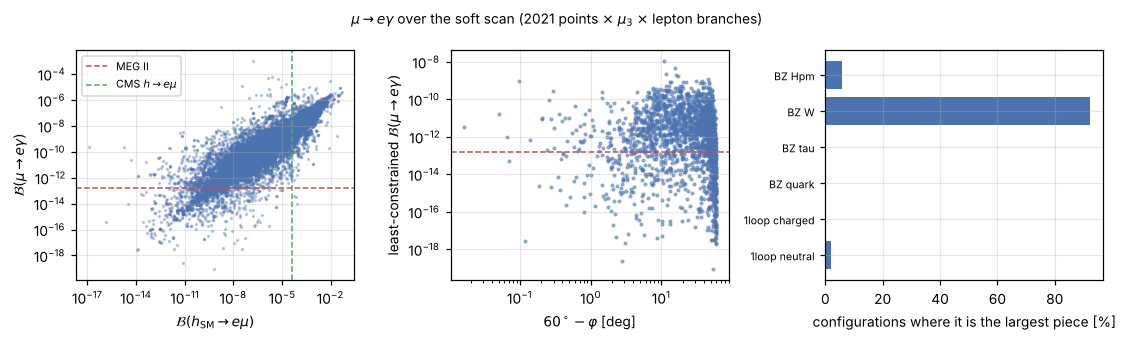
\includegraphics[width=\textwidth]{figures/meg_scan.png}
\caption{Left: $\mathcal B(\mu\to e\gamma)$ against the SM-like $\mathcal B(h\to e\mu)$ per
configuration (40\,000 sampled), with the MEG~II and CMS limits dashed. Middle: the
least-constrained configuration of each scalar point against the vacuum misalignment.
Right: which piece of the amplitude is largest, by share of configurations.}
\label{fig:scan}
\end{figure}

\textbf{What drives it.} The Barr--Zee $W$ loop through the SM-like Higgs is the largest
piece in 92\% of configurations, the $H^\pm$ Barr--Zee loop in 5.8\%, and the one loop in
about 2\%. The SM-like state's $e\mu$ coupling is pure non-vacuum admixture (previous
report), so the survivors are the more aligned points: their median $1-\kappa_V^2$ is
$8.3\times10^{-4}$, compared with $2.4\times10^{-3}$ overall. No $\mu_3$ window or
lepton-branch kind is singled out. MEG-allowed configurations span the whole $|\mu_3|$ axis
and all three branch kinds. Being close to $\varphi=\pi/3$ does not protect a point
(Fig.~\ref{fig:scan}, middle). In the scan the free soft terms break the $\mathbb Z_2$
whatever $\varphi$ is, so $\varphi$ is not its order parameter.

\textbf{Robustness.} The two least certain inputs are the quark couplings (an ansatz, and
the top loop interferes destructively with the $W$ loop) and the 14\% $W$-loop gap. Each
configuration carries three variants built from the same amplitudes:

\begin{center}
\begin{tabular}{lc}
\toprule
variant & scalar points allowed by MEG~II\\
\midrule
baseline & \nMEGallowed{}\\
no quark Barr--Zee & \nMEGnoQuark{}\\
quark couplings with opposite sign & \nMEGtopFlip{}\\
$W$ loop scaled to \cite{HKZ13}'s 0.11 & \nMEGwHKZ{}\\
\bottomrule
\end{tabular}
\end{center}

The count moves by about 25\%, and the conclusion that MEG~II removes most of the scalar
sector does not.

\section{Open questions}

\begin{enumerate}\itemsep4pt
\item \textbf{Missing two-loop pieces:} \cite{HKZ13}'s set C, and the $\phi Z\gamma$ and
$H^\pm W^\mp\gamma$ Barr--Zee diagrams. The variants above suggest their effect on the
point count is of the same order as the quark uncertainty, but they are not computed.
\item \textbf{The quark sector per point}, to replace the Barr--Zee quark ansatz. The same
input is missing from $R_{\gamma\gamma}$.
\item \textbf{An order parameter for the residual $\mathbb Z_2$} in the soft vacuum: a
combination of soft terms rather than $\varphi$. It would turn the near-zero of
\S\ref{sec:exact} into a scan variable.
\item \textbf{$\mu\to3e$ and $\mu$--$e$ conversion} share this dipole and add contact terms.
\textbf{$\tau\to\mu\gamma$ and $\tau\to e\gamma$} need only the flavour indices of
\texttt{radiative.py} generalized.
\end{enumerate}

\begin{thebibliography}{9}

\bibitem{MEGII25} MEG~II Collaboration,
\emph{New limit on the $\mu^+\to e^+\gamma$ decay with the MEG~II experiment} (2025),
\href{https://arxiv.org/abs/2504.15711}{arXiv:2504.15711}.

\bibitem{OST16} Y.~Omura, E.~Senaha and K.~Tobe,
\emph{$\tau$- and $\mu$-physics in a general two Higgs doublet model with $\mu-\tau$ flavor
violation}, Phys.\ Rev.\ D \textbf{94}, 055019 (2016),
\href{https://arxiv.org/abs/1511.08880}{arXiv:1511.08880}.

\bibitem{HKZ13} R.~Harnik, J.~Kopp and J.~Zupan,
\emph{Flavor violating Higgs decays}, JHEP \textbf{03} (2013) 026,
\href{https://arxiv.org/abs/1209.1397}{arXiv:1209.1397}.

\bibitem{Ilisie15} V.~Ilisie,
\emph{New Barr-Zee contributions to $(g-2)_\mu$ in two-Higgs-doublet models},
JHEP \textbf{04} (2015) 077,
\href{https://arxiv.org/abs/1502.04199}{arXiv:1502.04199}.

\bibitem{Lavoura03} L.~Lavoura,
\emph{General formulae for $f_1\to f_2\gamma$}, Eur.\ Phys.\ J.\ C \textbf{29}, 191 (2003),
\href{https://arxiv.org/abs/hep-ph/0302221}{hep-ph/0302221},
\href{https://doi.org/10.1140/epjc/s2003-01212-7}{doi:10.1140/epjc/s2003-01212-7}.

\bibitem{CMS21} CMS Collaboration,
\emph{Search for lepton-flavor violating decays of the Higgs boson in the $\mu\tau$ and
$e\tau$ final states in pp collisions at $\sqrt s=13$~TeV},
Phys.\ Rev.\ D \textbf{104}, 032013 (2021),
\href{https://arxiv.org/abs/2105.03007}{arXiv:2105.03007}.

\bibitem{CMS23} CMS Collaboration,
\emph{Search for the lepton-flavor violating decay of the Higgs boson and additional Higgs
bosons in the $e\mu$ final state in proton-proton collisions at $\sqrt s=13$~TeV},
Phys.\ Rev.\ D \textbf{108}, 072004 (2023),
\href{https://arxiv.org/abs/2305.18106}{arXiv:2305.18106}.

\end{thebibliography}

\end{document}
